%%%%%%%%%%%%%%%%%%%%%%%%%%%%%%%%%%%%%%%%%%%%%%%%%%%%%%%%%%%%%%%%%%%%
%% I, the copyright holder of this work, release this work into the
%% public domain. This applies worldwide. In some countries this may
%% not be legally possible; if so: I grant anyone the right to use
%% this work for any purpose, without any conditions, unless such
%% conditions are required by law.
%%%%%%%%%%%%%%%%%%%%%%%%%%%%%%%%%%%%%%%%%%%%%%%%%%%%%%%%%%%%%%%%%%%%
\documentclass{beamer}

\usepackage[english]{babel}
\usepackage[utf8]{inputenc}
\usepackage[T1]{fontenc}
\usepackage{booktabs}
\usetheme[workplace=ics]{MU}

% added by Jamie
\usepackage{svg}
\usepackage{bm}

% FROM: https://castel.dev/post/lecture-notes-2/
\usepackage{import}
\usepackage{xifthen}
\usepackage{pdfpages}
\usepackage{transparent}

% \newcommand{\incfig}[1]{%
    % \def\svgwidth{0.9\columnwidth}
    % \import{./imgs/}{#1.pdf_tex}
% }
%

\usepackage{bbding}
% \setbeamertemplate{itemize items}[square]
\newcommand\Wider[2][3em]{%
\makebox[\linewidth][c]{%
  \begin{minipage}{\dimexpr\textwidth+#1\relax}
  \raggedright#2
  \end{minipage}%
  }%
}
\usepackage{multimedia}
% \usefonttheme[onlymath]{serif}
% \usefonttheme{professionalfonts}
\usepackage{framed}
\newcommand{\mybox}[3]{{\color{#1}\framebox{\color{#2}#3}}}
\usepackage[skins,listings,breakable,many]{tcolorbox}
% \lstset{basicstyle=\footnotesize, columns=fullflexible}
% \lstset{basicstyle=\footnotesize, backgroundcolor=\color{lightgray}}
% \lstset{basicstyle=\footnotesize, showstringspaces=false}
\lstset{basicstyle=\scriptsize, showstringspaces=false}

\usepackage{mdframed}

\newcommand\blfootnote[1]{%
  \begingroup
  \renewcommand\thefootnote{}\footnote{#1}%
  \addtocounter{footnote}{-1}%
  \endgroup
}

\begin{document}

\setbeamertemplate{caption}{\raggedright\insertcaption\par}

% \title[]{An Investigation into Cell-Centred vs Cell-Vertex FVM} %% that will be typeset on the
\title[]{Can I make regression with fancy lingo beat Eilmer?} %% that will be typeset on the

% \subtitle[]{A "Lightning" Talk} %% title page.
\subtitle[]{Machine Learning of Bow Shocks} %% title page.
% \subtitle{} %% title page.
\author[]{Jamie Border}
% \title[Short Presentation Title]{Full Presentation Title}
% \subtitle[Short Presentation Subtitle]{Full Presentation Subtitle}
% \author[J.\,Doe]{Jane Doe \\ personal-id@mail.muni.cz}
% \institute{School of Mechanical and Mining Engineering, The University of Queensland}
\institute{A Lightning Talk}
\date{November 18th, 2022}
% \date{\today}
% \subject{Presentation Subject}
% \keywords{the, presentation, keywords}

% \begin{frame}[plain]
% \maketitle
% \end{frame}
  \frame{\maketitle}
  % \maketitle


  % \begin{darkframes}

    \begin{frame}{\mybox{green}{blue}{Problem definition}}
        \vspace{-0.1cm}
        \begin{figure}
            % \includesvg[width=0.4\textwidth]{./imgs/shock-fitting.svg}
            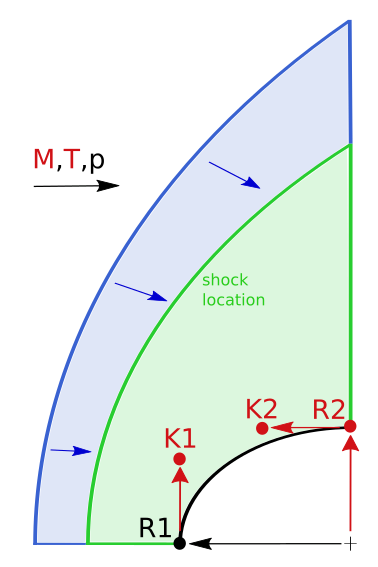
\includegraphics[width=0.4\textwidth]{./imgs/shock-fitting.png}
        \end{figure}
    \end{frame}

    \begin{frame}{\mybox{green}{blue}{Randomly generated bodies and shock-fit bow shocks}}
        \vspace{-0.5cm}
        \begin{columns}
            \begin{column}{0.5\textwidth}
                % \vspace{-2.0cm}
                \begin{figure}
                    % \includesvg[width=0.4\textwidth]{./imgs/rand_shocks.svg}
                    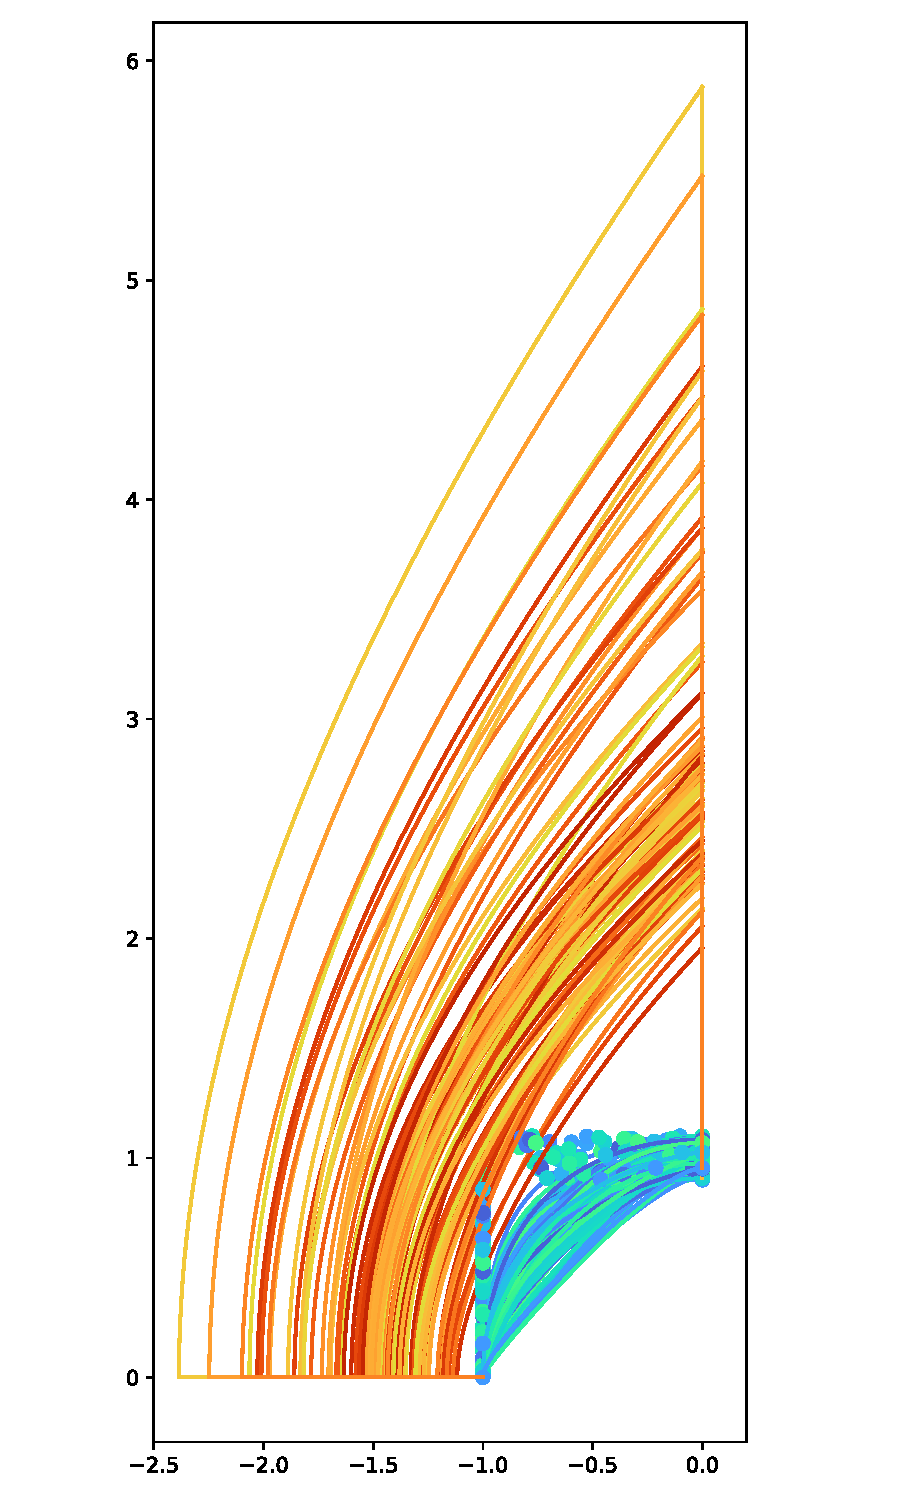
\includegraphics[width=0.8\textwidth]{./imgs/rand_shocks.pdf}
                    % \caption{centroidal dual}
                \end{figure}
            \end{column}
            % \hspace{-0.5cm}
            \begin{column}{0.5\textwidth}  %%<--- here
                \vspace{0.5cm}
                \begin{figure}
                    % \includesvg[width=0.4\textwidth]{./imgs/rand_shocks_zoom.svg}
                    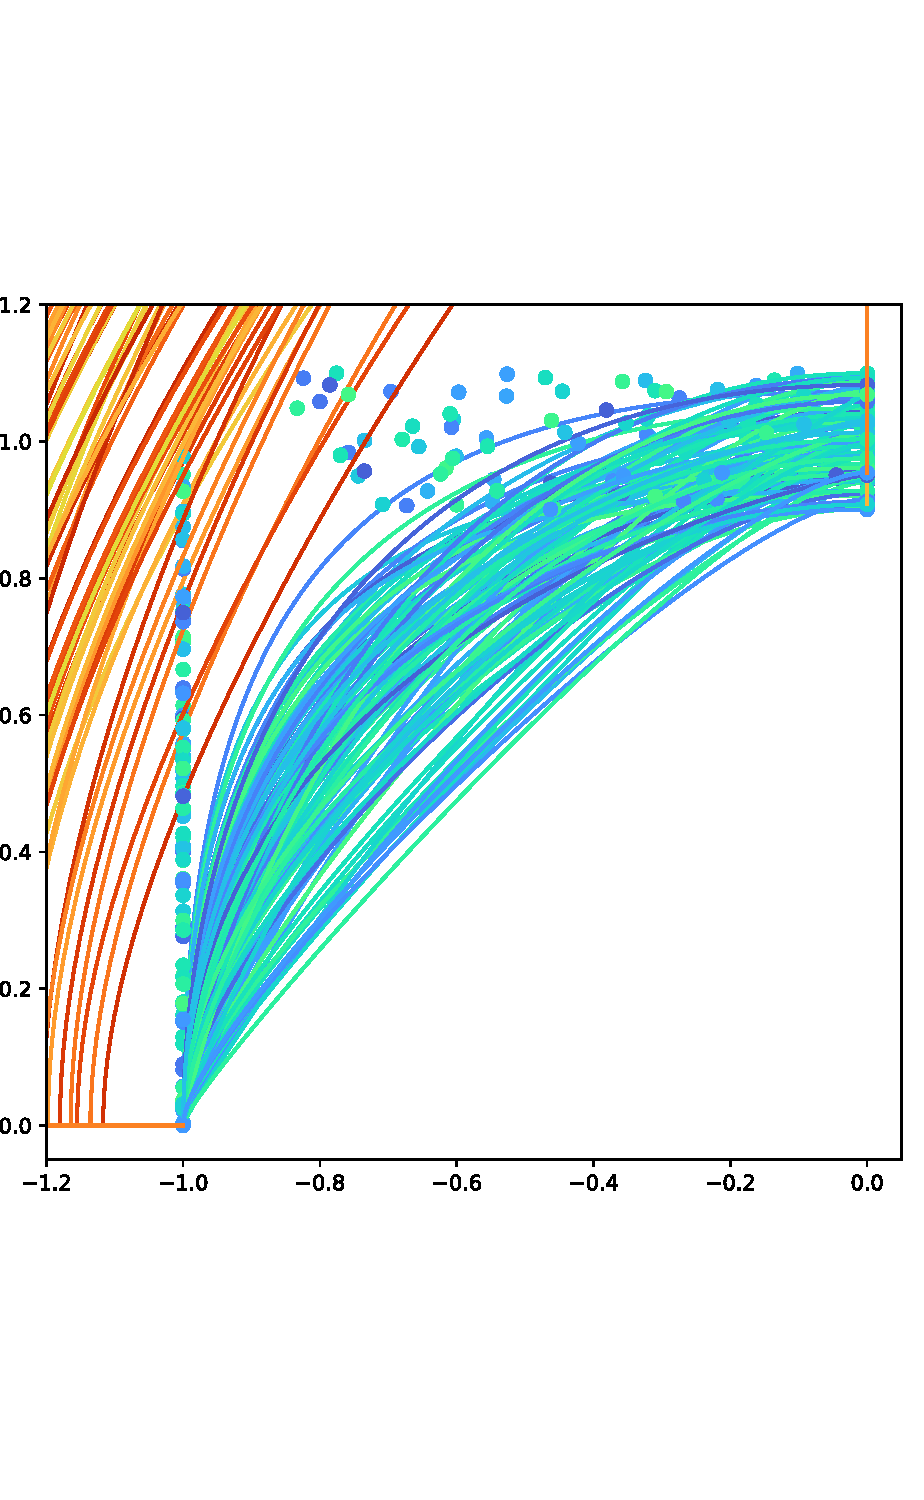
\includegraphics[width=1.0\textwidth,trim=0 0 0 100,clip]{./imgs/rand_shocks_zoom.pdf}
                    % \caption{median dual}
                \end{figure}
            \end{column}
        \end{columns}
    \end{frame}

    \begin{frame}{\mybox{green}{blue}{Mapping from cartesian to polar coordinates}}
        \vspace{-0.2cm}
        \begin{figure}
            \def\svgwidth{0.9\columnwidth}
            \import{./imgs/}{mapping.pdf_tex}
        \end{figure}
    \end{frame}

    \begin{frame}{\mybox{green}{blue}{Fitting to shock data}}
        \vspace{-0.5cm}
        \begin{align*}
            r(\theta)=\sum_{k=0}^{m}a_k\theta^k\, , \;\;\;\; \frac{d r(\theta)}{d \theta} = \sum_{k=1}^{m}ka_k\theta^{k-1}\, , \;\;\;\;\theta=[0,\pi/2]
        \end{align*}
        Least-squares fit,
        \begin{align*}
            I = \sum_{i=1}^{N}\left|\left|r(\theta_i) - r_i\right|\right|^2;
        \end{align*}
        % in matrix form, solving $\bm{A}\bm{x} = \bm{b}$, giving
        in matrix form, solving $I = (\bm{A}\bm{x} - \bm{b})^2$, giving
        \begin{align*}
            \bm{A}^T\bm{A}\bm{x} = \bm{A}^T\bm{b},
        \end{align*}
        or if including gradient terms as constraints
        \begin{align*}
\begin{bmatrix}
    \bm{A}^T\bm{A} & \bm{C}^T\\
    \bm{C}         & \bm{0}
\end{bmatrix}
\begin{bmatrix}
    \bm{x}\\
    \bm{\lambda}        
\end{bmatrix}
=
\begin{bmatrix}
    \bm{A}^T\bm{b}\\
    \bm{d}
\end{bmatrix}.
        \end{align*}
    \end{frame}

    \begin{frame}{\mybox{green}{blue}{ML}}
        \vspace{-1.5cm}
        \begin{figure}
            \def\svgwidth{0.9\columnwidth}
            \import{./imgs/}{ml.pdf_tex}
        \end{figure}
    \end{frame}

    \begin{frame}{\mybox{green}{blue}{Example fit in polar coordinates}}
        \vspace{-0.1cm}
        \begin{figure}
            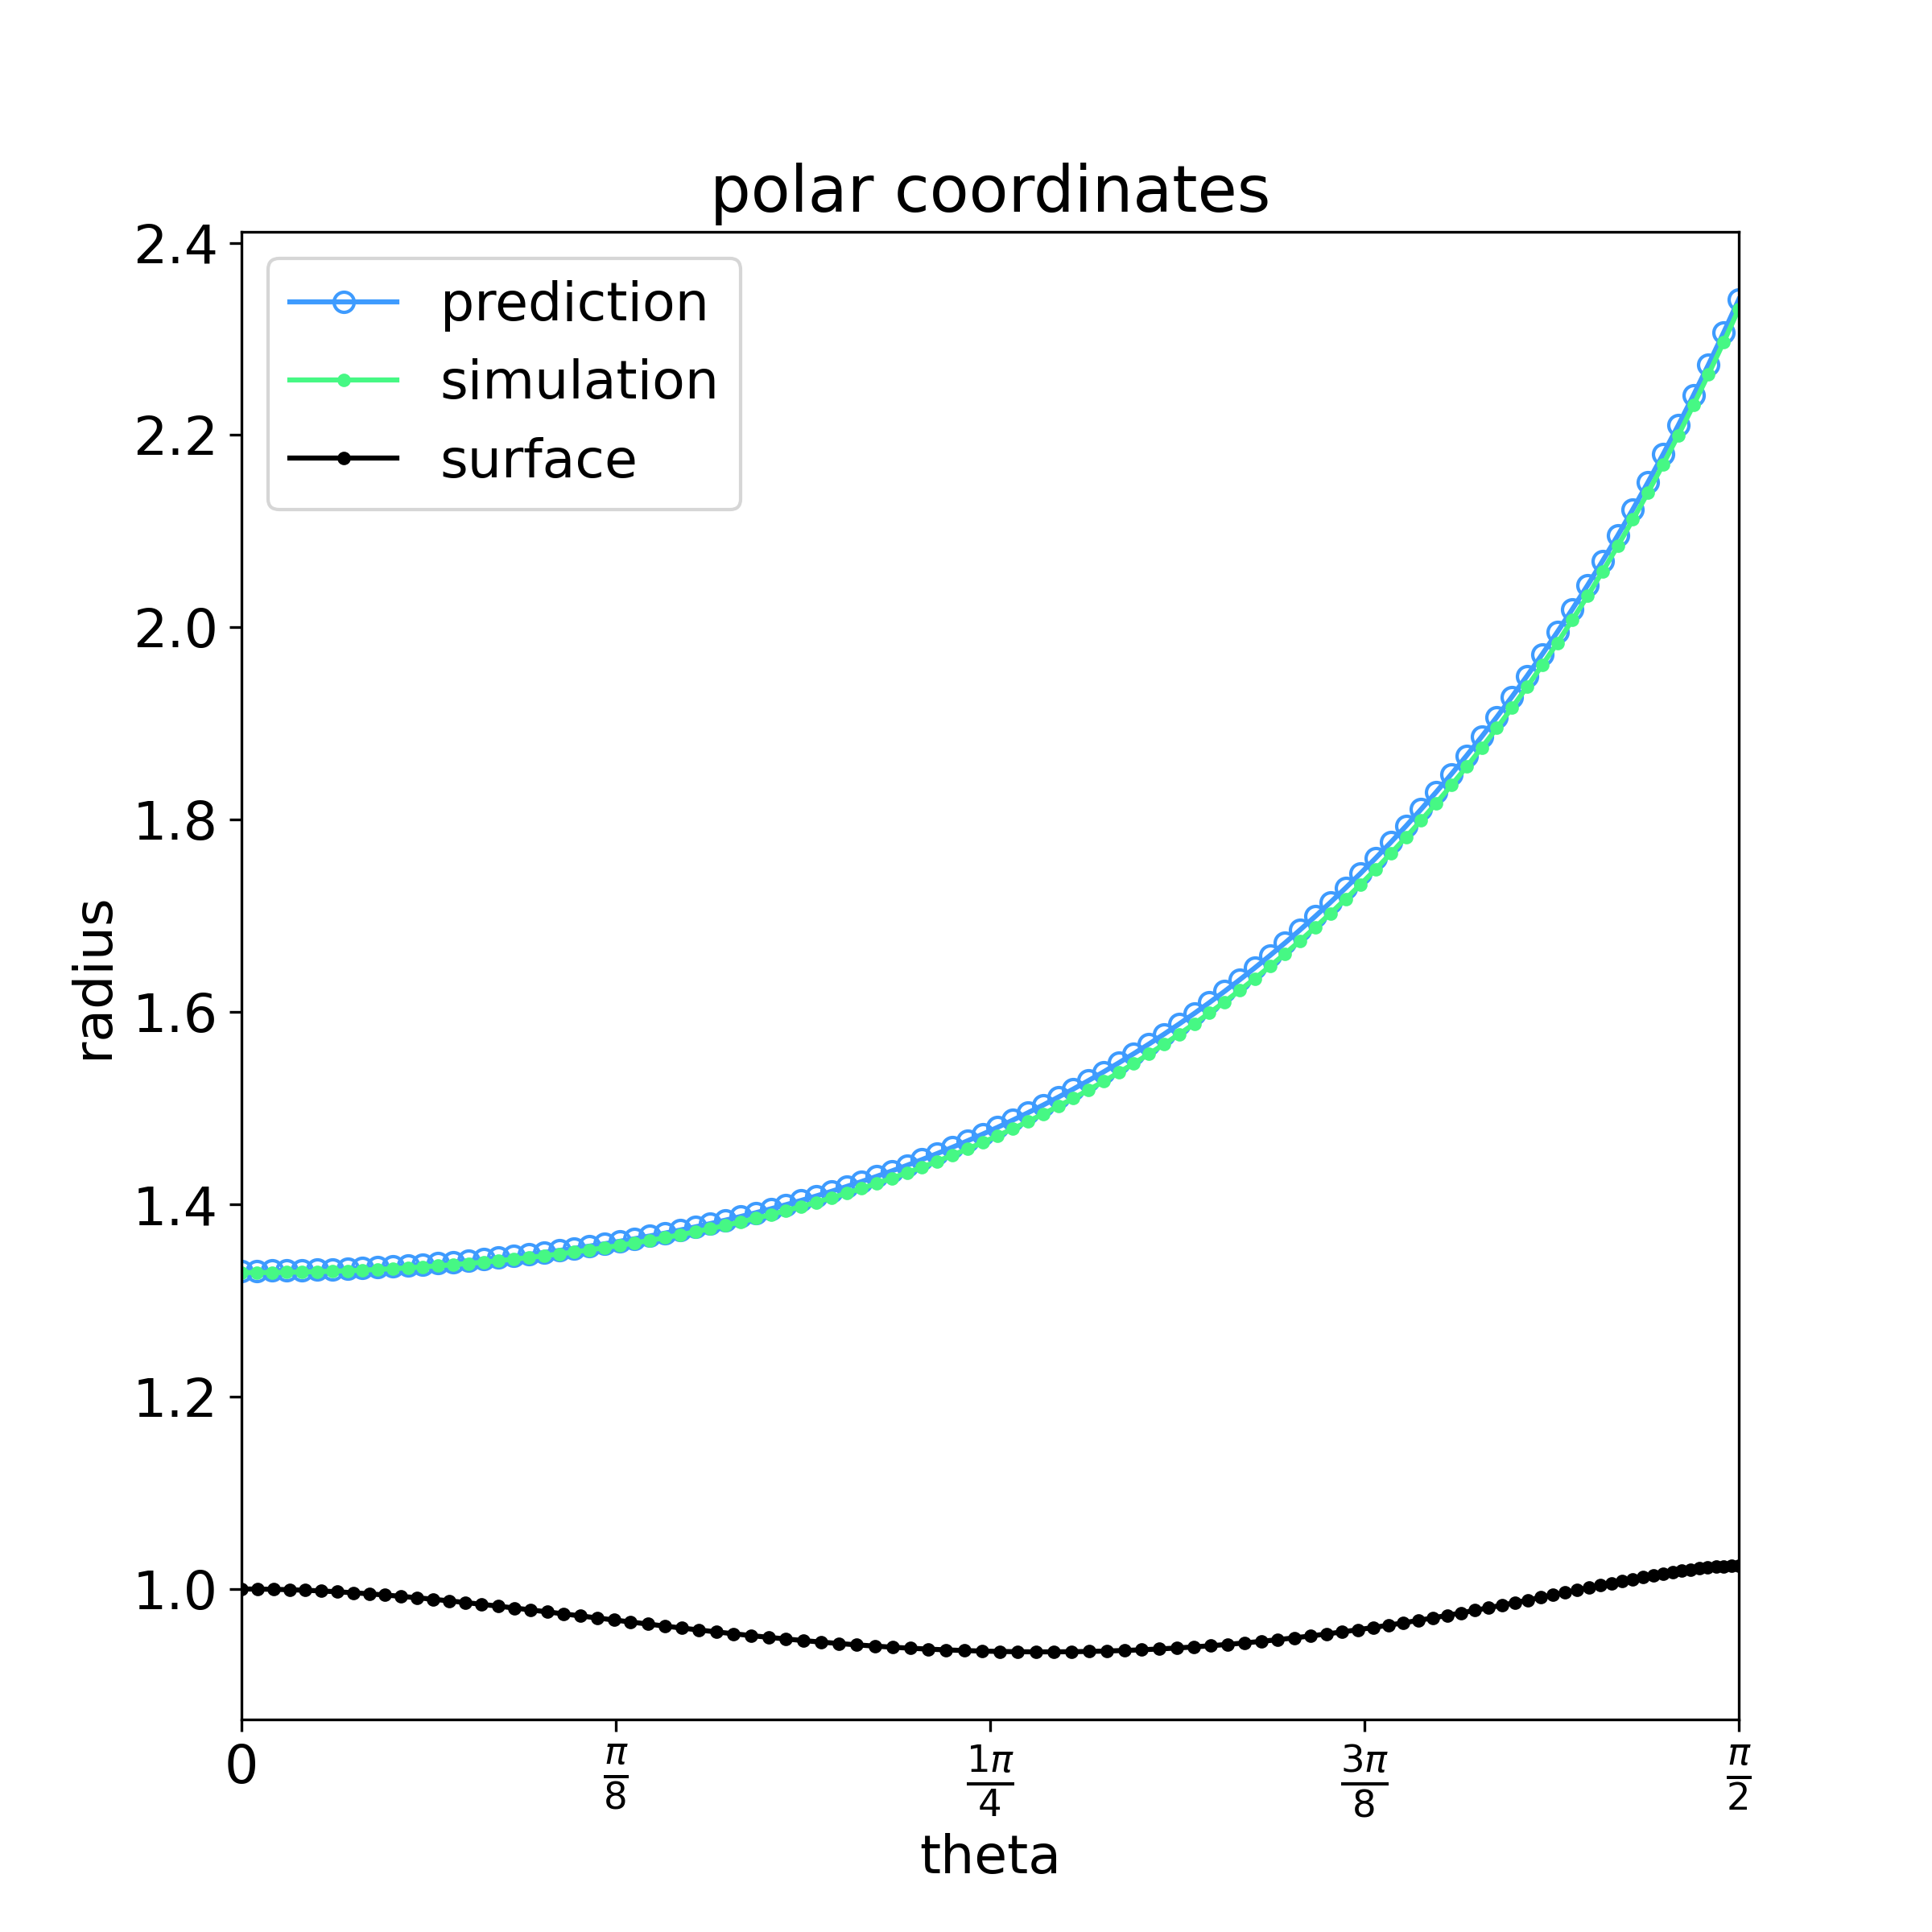
\includegraphics[width=0.8\textwidth,trim=0 0 0 65,clip]{../ml/examples/ex2/pred_polar.png}
        \end{figure}
    \end{frame}

    \begin{frame}{\mybox{green}{blue}{Example fit in cartesian coordinates}}
        \vspace{-0.1cm}
        \begin{figure}
            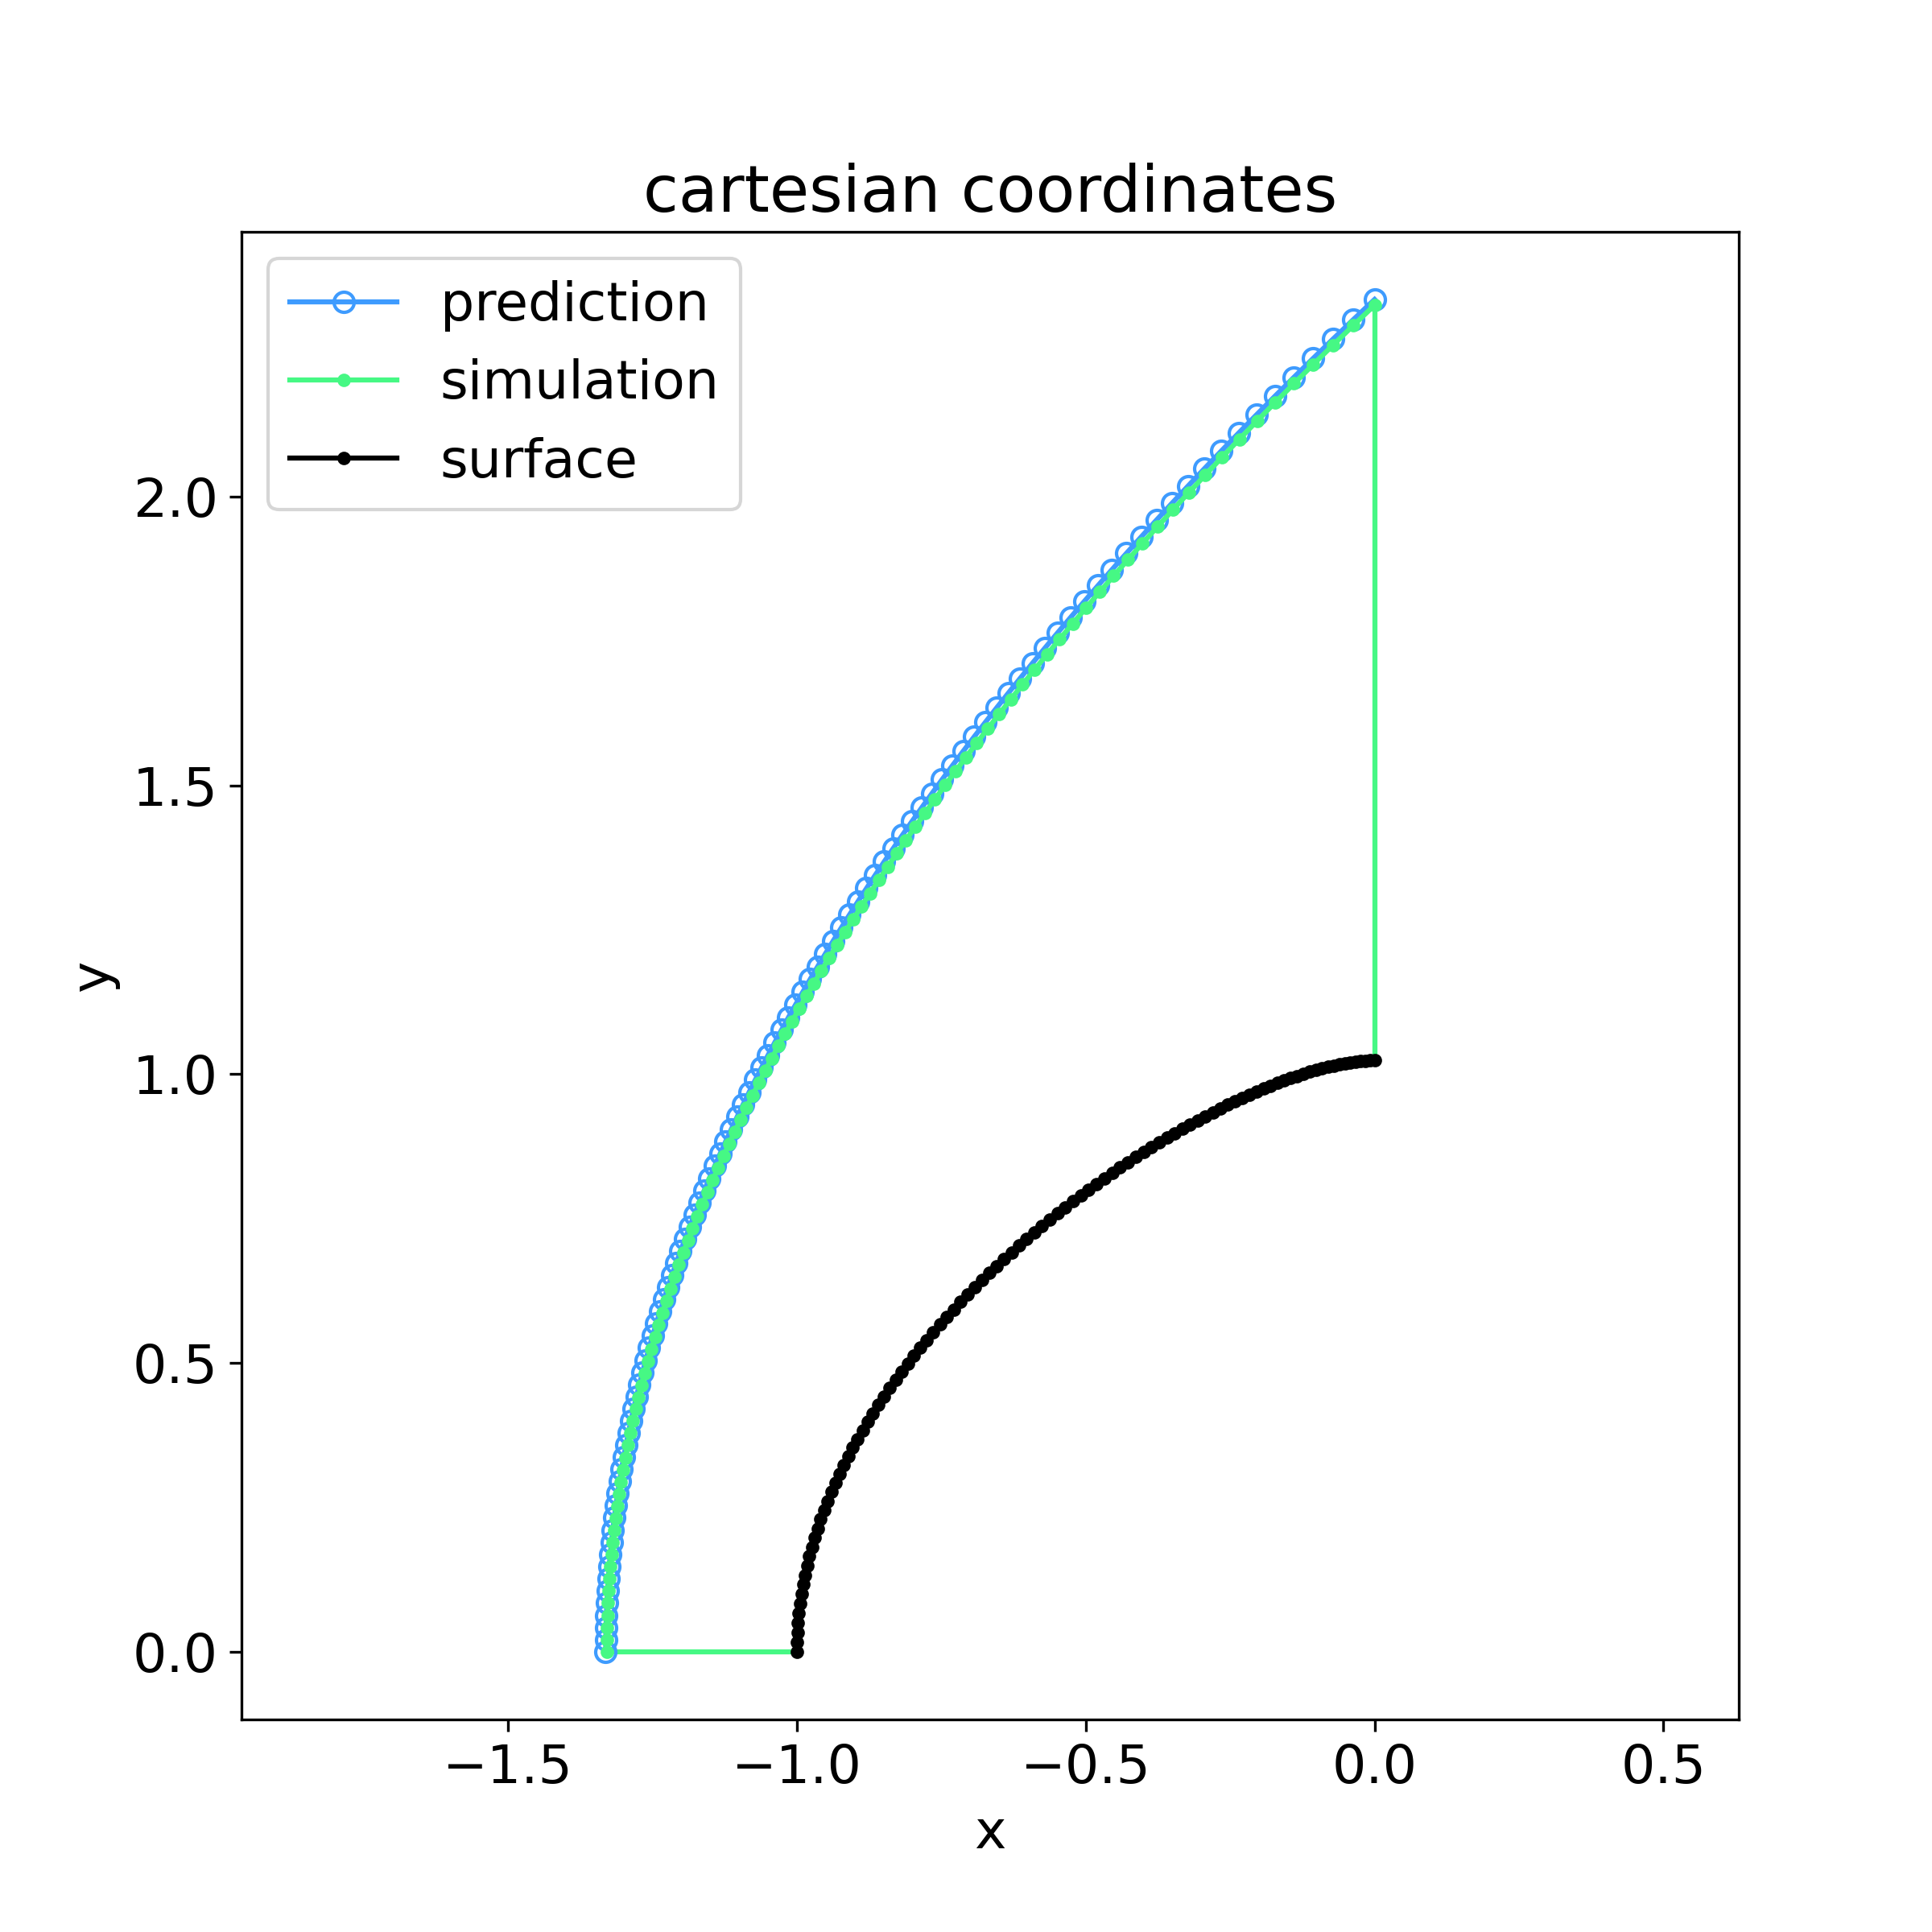
\includegraphics[width=0.8\textwidth,trim=0 0 0 65,clip]{../ml/examples/ex2/pred_cartesian.png}
        \end{figure}
    \end{frame}

    %%%%%%%%%%%%%%%%%%%%%%%%%%%%%%%%%%%%%%%%%%%%%%%%%%%%%%%%%%%%%%%%%%%%%

  % \end{darkframes}
\end{document}
